\chapter{Results}%
\label{chap:results}
\textit{This chapter presents the test results that test and challenge the proposed method. Three types of test are introduced which are custom made benchmark tests, randomisation tests and test taken including and excluding the \ac{kgraph}. The test results provide evidence that support the effectiveness of the proposed method. This chapter starts by introducing \textbf{method metrics} that indicate how a task has been executed by the proposed method in \cref{sec:proposed_method_metrics}. Then the three types of test are presented in \cref{sec:benchmark_tests,sec:randomisation,sec:kgraph_on_off}. A comparison is made with the state-of-the-art methods in \cref{sec:compare_with_related_papers}, the chapter is finalised with a discussion about the results in \cref{sec:discussion}.\bs}

\paragraph{The Simulation Environment}
Testing in a simulation environment has been done using the URDF Gym Environment~\cite{spahn_urdfenvironment_2022}, a 100\% python environment build upon the PyBullet library~\cite{coumans_pybullet_2016}. The code created during the thesis can be found on \href{https://gitlab.tudelft.nl/airlab-delft/msc_projects/msc_gijs_groote}{GitLab} and \href{https://github.com/GijsGroote/semantic-thinking-robot}{GitHub}. Experiments ran on standard TU Delft laptop: HP ZBook Studio x360 G5, running OS: Ubuntu 22.04.1 LTS x86\_64, CPU: Intel i7-8750H (12) @ 4.100GHz, GPU: NVIDIA Quadro P1000 Mobile.\bs
The simulation environment provides many different robots, 2 simple robots are selected to perform tests, they are displayed in \cref{fig:example_robots}, and various objects are displayed in \cref{fig:example_objects}.


\todo[inline]{The results will be made in a while, wait for a moment while we try to make sense of the almost-existing results}

\section{Proposed Method Metrics}%
\label{sec:proposed_method_metrics}
The results are measured in method metrics, not to be confused with the monitoring metrics in \cref{sec:monitoring_metrics} or the edge metrics in \cref{subsec:edge_metrics}. The results are interseting, but most interesting is the progression of the method metrics over time. As will be shown, the effect of learning can be measured by investigating tracking the method metrics over time. Furthermore, the method metrics will be used to compare the proposed method to relative state-of-the-art papers. First the method metrics are presented in~\cref{table:proposed_method_metrics} with corresponding argumentation on the relevance of the metric.\bs

\begin{table}[htb!]
\centering
\begin{tabular}[t]{p{4cm} p{10cm}}
Total Average\newline \acl{PE} & The total average \ac{PE} is created by averaging over every hypothesis' average \ac{PE} in a \ac{hgraph}. Since the \ac{PE} is high when unexpected behaviour occurs, seeing the total average \ac{PE} lower would indicate the robot encounters less unexpected behaviour, indicating the robot is learning.\\
Total Average\newline \acl{TE}& The total average \ac{TE} is created by averaging over every hypothesis' average \ac{TE} in a \ac{hgraph}. Seeing the total average \ac{TE} lower over time would indicate the robot is selecting better suitable controllers and system models, indicating the robot is learning.\\
Final positions and\newline displacement errors & The final position and displacement error is a metric which how a controller performs. This thesis does not create or investigate controllers, but it is interesting to see why different controllers are preferred for different objects. The final position and displacement error could be the cause.\\
The ratio between the nubmer of hypothesis and the number of tasks & Expected is that whilst learning system models, the hypothesis created will be more effective. Thus the ratio between the total number of hypotheses and the total number of tasks is expected to lower with new knowledge.\\
The ratio between the number of successfull and the nubmer of total edges in \ac{kgraph} & When the \ac{kgraph} improves recommending a controller and system model, the ratio between successful edges and total edges is expected to increase because, with better recommendations, more edges will be succesfully completed.\\
task completion time =\newline runtime + planning time& If equal tasks are given multiple times, the total task completion time should drop pretty drastically. Multiple factors help to lower the task completion time, firstly system identification has to be performed only once, and there is no need to lose time on redoing system identification. Secondly, the \ac{hgraph} is expected to improve generated hypothesis, or better said, the same mistake should not be made multiple times, resulting in fewer failing hypotheses and lowering task completion time.\\
\end{tabular}
\caption{Proposed method metrics used to compare the proposed method with the state-of-the-art methods.}\label{table:proposed_method_metrics}
\end{table}

\newpage
\section{Benchmark Tests}%
\label{sec:benchmark_tests}
Three benchmark test are now presented, starting with the blockade task. A large part of the proposed method is system identification, for testing however no system identification is performed. Instead a number of hardcoded system models are used, the \ac{kgraph} finds which system model is the best choice for an object over time. Where the best choice is defined using the edge metrics discussed in \cref{subsec:edge_metrics}. Now these hardcoded system models are shortly discussed.\bs

\todo[inline]{define nonlinear-drive-model}
\todo[inline]{define lti-drive-model}
\todo[inline]{define nonlinear-push-model-2}
\todo[inline]{define nonlinear-push-model-2}

\paragraph{Blockade}
\begin{figure}[H]
    \centering
    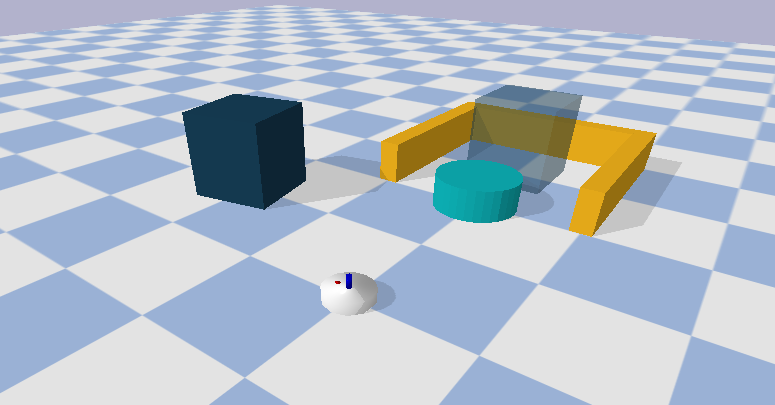
\includegraphics[width=13cm]{figures/tests/blockade}
    \caption{The blockade environment with the target ghost position for the blue box.}%
    \label{fig:benchmark_blockade}
\end{figure}

The blockade task neatly shows that the \ac{halgorithm} uses the backward search technique. First the \ac{halgorithm} plans to push the box directly to the target position, then it realises a blocking object must first be moved to free the path. It makes the mistake of pushing the unmovable wall, then it succeeds in pushes the movable cylinder out of the way. The \ac{kgraph} then ensures that this mistake will not occur again because is remebered that the wall is immovable. Over time the \ac{kgraph} indicates that it prefers to use the \ac{MPPI} controller with the nonlinear-push-model-2 to push both the box and the cylinder object.\bs
\todo[inline]{is nonlinear-push-model-2 still the preferred model?}

\todo[inline]{results for running the blockade environment multiple times}

\todo[inline]{duck or cylinder, you've told the reader that there would only be boxes and cylinders}
\todo[inline]{tell the reader there also is a duck now, because that duck is really nice I think}

\paragraph{Swap}
\begin{figure}[H]
    \centering
    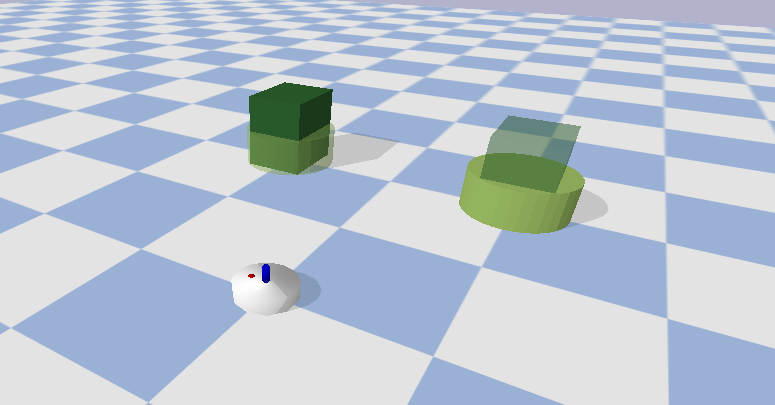
\includegraphics[width=13cm]{figures/tests/swap}
    \caption{The swap environment, the robot is tasked with swapping the positions of the cylinder and the box.}%
    \label{fig:benchmark_swap}
\end{figure}


\paragraph{Surrounded}
\begin{figure}[H]
    \centering
    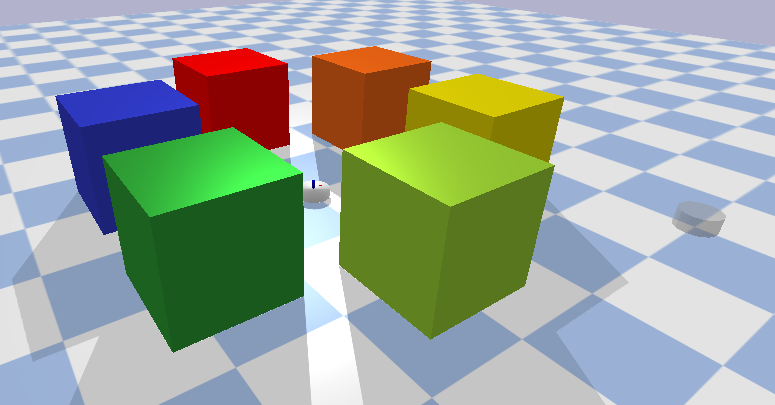
\includegraphics[width=13cm]{figures/tests/surrounded}
    \caption{The surround environment, the robot should escape the surrounding enclosure. All box objects are unmovable obstacles with the exception of the green box.}%
    \label{fig:benchmark_surround}
\end{figure}

\section{Randomisation}%
\label{sec:randomisation}
The Randomised environment.\bs
\todo[inline]{write some rand env intro}

\begin{figure}[H]
    \centering
    \begin{subfigure}{\textwidth}
    \centering
    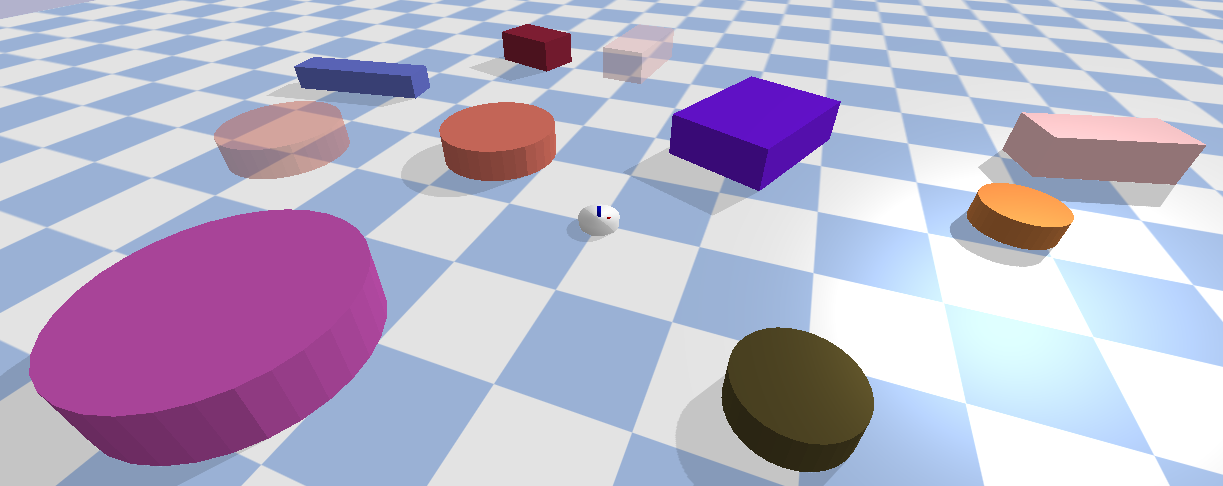
\includegraphics[width=1.0\textwidth]{figures/tests/random_1}
    \end{subfigure}
    \begin{subfigure}{\textwidth}
    \centering
    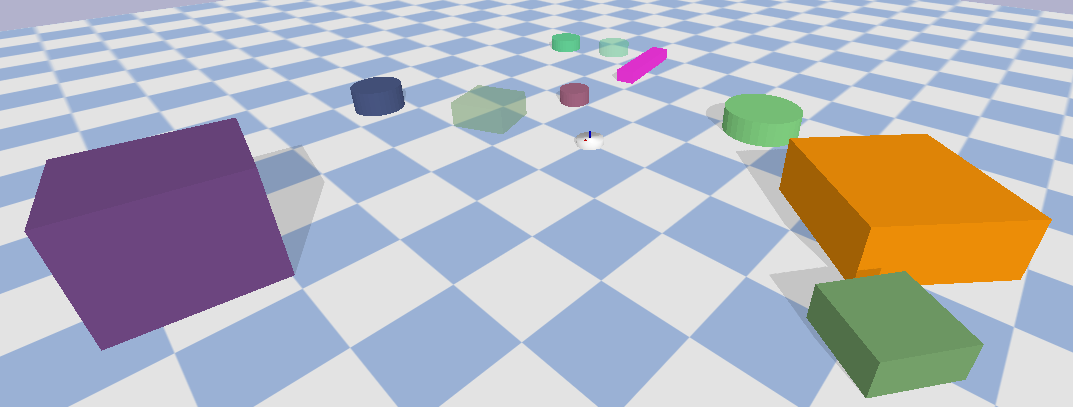
\includegraphics[width=1.0\textwidth]{figures/tests/random_2}
    \end{subfigure}
    \caption{Two random environment with target ghost configurations for a task that contains 2 subtasks.}%
    \label{fig:random_environnment}
\end{figure}

\begin{figure}[H]
    \centering
    \begin{subfigure}{.49\textwidth}
    \centering
    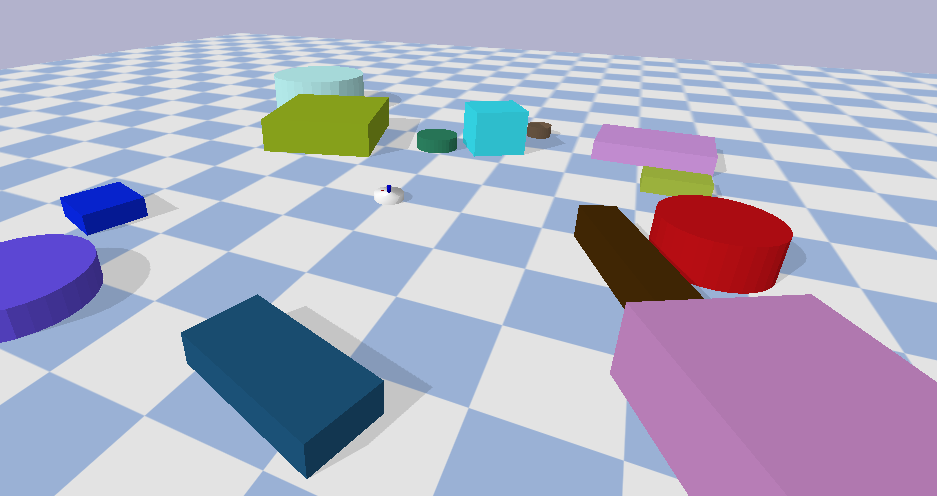
\includegraphics[width=\textwidth]{figures/tests/random1}
    \end{subfigure}
    \hfill
    \begin{subfigure}{.49\textwidth}
    \centering
    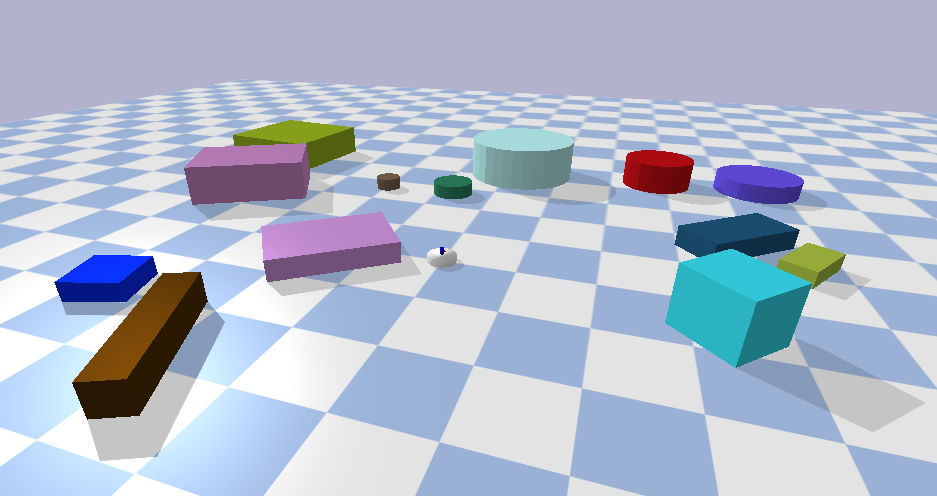
\includegraphics[width=\textwidth]{figures/tests/random2}
    \end{subfigure}

    \vspace{0.2cm}
    \begin{subfigure}{.49\textwidth}
    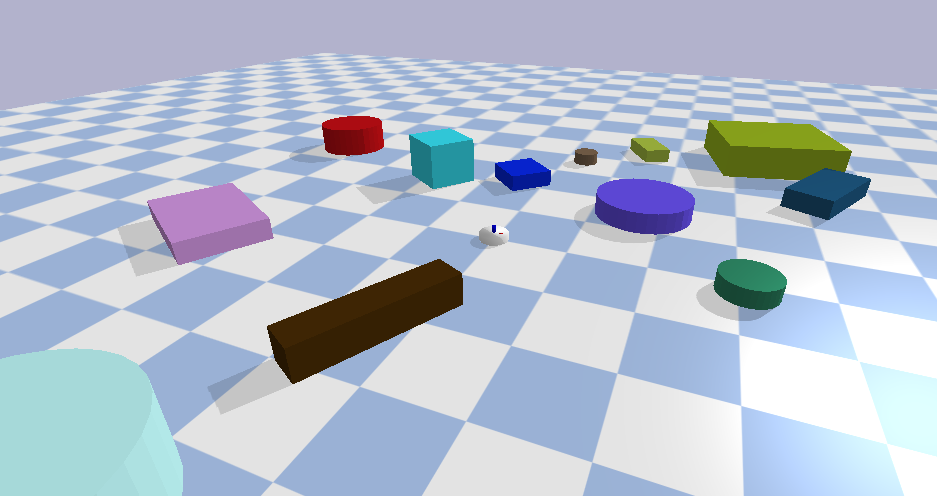
\includegraphics[width=\textwidth]{figures/tests/random3}
    \end{subfigure}
    \hfill
    \begin{subfigure}{.49\textwidth}
    \centering
    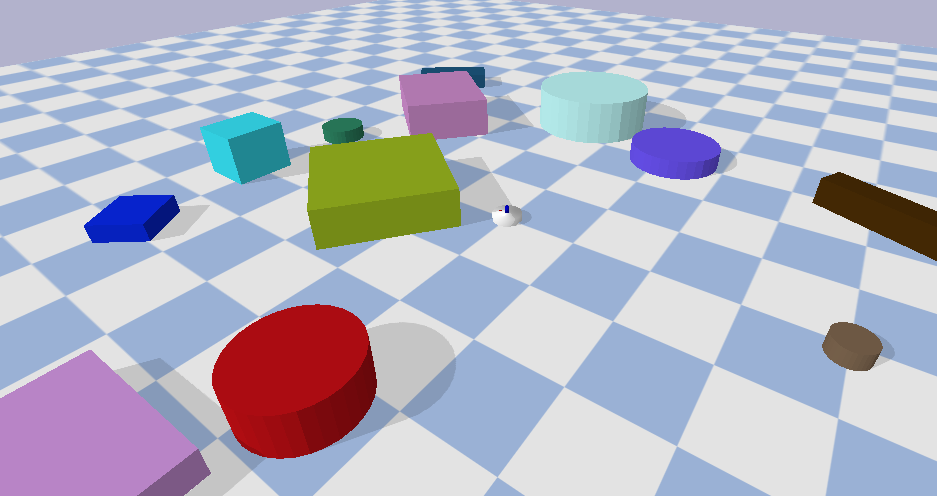
\includegraphics[width=\textwidth]{figures/tests/random4}
    \end{subfigure}
    \caption{A random environments that is reshuffled 4 times. Target ghost configurations are not shown.}
    \label{fig:random_environment_reshuffle}
\end{figure}

% \section{Knowledge Graph On/Off}%
% \label{sec:kgraph_on_off}

\section{Comparison with related papers}%
\label{sec:compare_with_related_papers}

The papers to compare with:\newline

\citefield{sabbaghnovin_model_2021}{title}\\

\cite{sabbaghnovin_model_2021}, 
\todo[inline]{See the paper for tests to reproduce with my hgraph}


\citefield{novin_dynamic_2018}{title}\\
\cite{novin_dynamic_2018}
The following \cite{novin_dynamic_2018} citation is here because it is a refered to from \cite{sabbaghnovin_model_2021} many times




\section{Discussion}%
\label{sec:discussion}
